\documentclass[xcolor=table]{beamer}
\mode<presentation>
\usetheme{CambridgeUS}
\usepackage[russian]{babel}
\usepackage[utf8]{inputenc}
\usepackage[T2A]{fontenc}
\usepackage{sansmathaccent}
\usepackage{verbatim}
\usepackage{alltt}
\usepackage[table]{xcolor}
%\linespread{0.8}

\usepackage{minted}
\usepackage{setspace}

\pdfmapfile{+sansmathaccent.map}
\title[Язык C]{Управление процессами}
\author{Наумов Д.А., доц. каф. КТ}
\date[30.10.2019] {Операционные системы и системное программное обеспечение, 2020}

\begin{document}

%ТИТУЛЬНЫЙ СЛАЙД
\begin{frame}
  \titlepage
\end{frame}
  
%СОДЕРЖАНИЕ ЛЕКЦИИ
\begin{frame}
  \frametitle{Содержание лекции}
  \tableofcontents  
\end{frame}

\section{Основные понятия}

\begin{frame}{Программы, процессы и потоки}
	\begin{block}{Бинарный модуль (программа, приложение)}
		компилированный, исполняемый код, находящийся в каком-либо хранилище данных, например на диске.
	\end{block}
	\begin{block}{Процесс}
		запущенная программа.
	\end{block}
	Процесс включает в себя:
	\begin{itemize}
		\item бинарный образ, загружаемый в память;
		\item подгрузку виртуальной памяти;
		\item ресурсы ядра (открытые файлы, выполнение требований по безопасности);
		\item запуск одного или нескольких потоков.
	\end{itemize}
	\textbf{Поток} - это одно из действий внутри процесса. Поток имеет собственный виртуализированный процессор, включающий в себя стек, состояние процессора, например регистры, а также командные указатели.
\end{frame}

\section{Идентификаторы процессов}

\begin{frame}{Идентификатор процесса}
	\begin{block}{Идентификатор процесса (process ID, pid)}
		уникальное (в любой конкретный момент времени) число, обозначающее процесс
	\end{block}
	\begin{itemize}
		\item процесс бездействия (idle process) - pid = 0;
	\end{itemize}
	\begin{block}{Процесс инициализации}
		первый процесс, который ядро выполняет во время запуска системы, pid = 1
	\end{block}
	\begin{itemize}
		\item /sbin/init - наиболее вероятное размещение процесса инициализации 
		\item /etc/init - следующее вероятное размещение процесса инициализации
		\item /bin/init - резервное размещение процесса инициализации
		\item /bin/sh - местонахождение оболочки Bourne, которую ядро пытается запустить
	\end{itemize}
\end{frame}

\begin{frame}{Идентификатор процесса}
	\begin{block}{pid\_t}
		С точки зрения программирования идентификатор процесса обозначается типом pid\_t, величина которого определяется в заголовочном файле <<sys/types.h>>. 
	\end{block}
	Выделение идентификатора процесса
	\begin{itemize}
		\item максимальное значение - /proc/sys/kernel/pid\_max
		\item идентификаторы назначаются линейно
		\item ранее исползованные индентификаторы не назначаются, пока не будет достигнуто pid\_max 
	\end{itemize}
\end{frame}

\begin{frame}{Иерархия процессов, пользователи, группы}
	Процесс, запускающий другой процесс, называется \textbf{родительским}; новый процесс, таким образом, является \textbf{дочерним}.
	\begin{itemize}
		\item каждый процесс запускается каким­либо другим процессом (кроме, разумеется, процессов инициализации). 
		\item каждый дочерний процесс имеет <<родителя>>. 
		\item идентификатор родительского процесса - \textbf{ppid}.
		\item каждый процесс принадлежит определенному \textbf{пользователю} и \textbf{группе}. Эти принадлежности используются для управления правами доступа к ресурсам. 
		\item каждый дочерний процесс наследует пользователя и группу, которым принадлежал родительский процесс.
		\item каждый процесс является также частью \textbf{группы процессов}. Дочерние процессы, как правило, принадлежат к тем же группам процессов, что и родительские.
	(Пример: \textit{ls | less}) 
	\end{itemize}
\end{frame}

\begin{frame}{Иерархия процессов, пользователи, группы}
	Для получения информации о процессах предназначена программа ps, поддерживающая большое количество опций.
	~
	Если вызвать ps без аргументов, то на экране появится список процессов, запущенных под текущим терминалом:
	\begin{figure}[h]
		\centering
		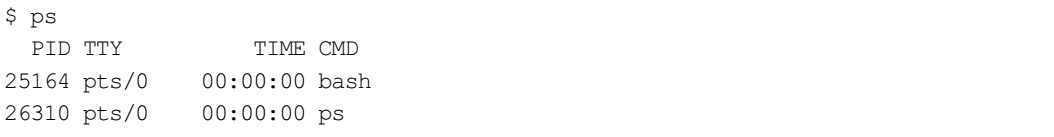
\includegraphics[scale=0.5]{images/lec07-pic22.png}
	\end{figure}
	\begin{itemize}
		\item Первый столбец (PID) - идентификатор процесса. 
		\item Второй и третий столбцы (TTY и TIME) пока не рассматриваемм. 
		\item В четвертом столбце (CMD) записывается имя исполняемого файла программы, запущенной внутри процесса.
	\end{itemize}
\end{frame}

\begin{frame}
	Если теперь запустить под оболочкой какую-нибудь программу, то она будет связана с текущим терминалом и появится в выводе программы ps. 
	\begin{figure}[h]
		\centering
		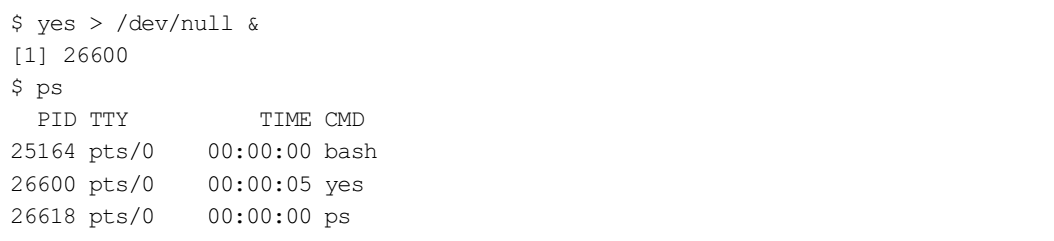
\includegraphics[scale=0.4]{images/lec07-pic23.png}
	\end{figure}
	Прерываем выполнение фоновой команды
	\begin{figure}[h]
		\centering
		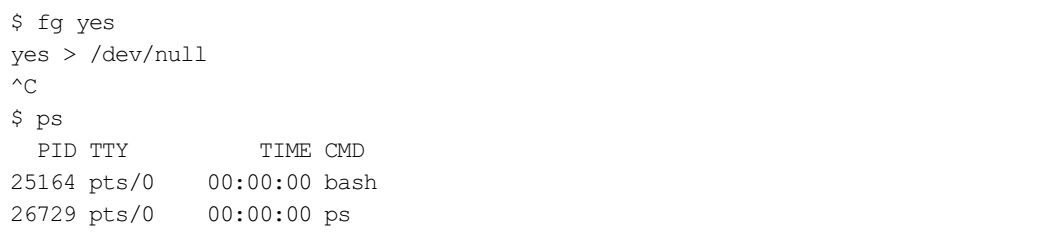
\includegraphics[scale=0.4]{images/lec07-pic24.png}
	\end{figure}
\end{frame}

\begin{frame}
	Если вызвать программу ps с опцией -f, то вывод пополнится несколькими новыми столбцами: 
	\begin{figure}[h]
		\centering
		
\includegraphics[scale=0.4]{images/lec07-pic25.png}
	\end{figure}
	\begin{itemize}
		\item В столбце PPID выводится идентификатор родительского процесса.
		\item Cтолбец UID (User IDentifier) в расширенном выводе программы ps содержит имя пользователя, от лица которого запущен процесс.
	\end{itemize}
\end{frame}

\begin{frame}
	Чтобы узнать числовой UID текущего пользователя, можно выполнить следующую команду:
	\begin{figure}[h]
		\centering
		
\includegraphics[scale=0.4]{images/lec07-pic26.png}
	\end{figure}
	Можно также узнать UID любого пользователя системы:
	\begin{figure}[h]
		\centering
		
\includegraphics[scale=0.4]{images/lec07-pic27.png}
	\end{figure}
	UID суперпользователя (с именем root в подавляющем большинстве случаев) всегда равен 0:
	\begin{figure}[h]
		\centering
		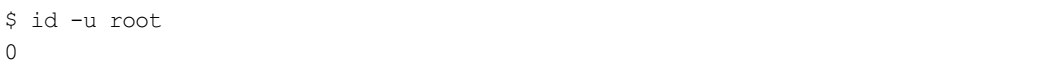
\includegraphics[scale=0.4]{images/lec07-pic28.png}
	\end{figure}
\end{frame}

\begin{frame}[fragile, shrink]
	\begin{minted}{c}
#include <sys/types.h>
#include <unistd.h>
#include <pwd.h>
#include <stdio.h>
#include <stdlib.h>

int main (void)
{
    int uid = getuid ();

    struct passwd * pwdp = getpwuid (uid);
    
    if (pwdp == NULL)
    {
        fprintf (stderr, "Bad username\n");
        return 1;
    }

    printf ("PID: %d\n", getpid ());
    printf ("PPID: %d\n", getppid ());
    printf ("UID: %d\n", uid);
    printf ("Username: %s\n", pwdp->pw_name);

    sleep (15);

    return 0;
}
	\end{minted}
\end{frame}

\begin{frame}[fragile]{Получение идентификатора процесса}
	Системный вызов \textit{getpid()} возвращает идентификатор вызывающего процесса:
	\begin{minted}{c}
	#include <sys/types.h>
	#include <unistd.h>
	pid_t getpid ();
	\end{minted}
	Cистемный вызов \textit{getppid()} возвращает идентификатор родителя вызывающего процесса:
	\begin{minted}{c}
	#include <sys/types.h>
	#include <unistd.h>
	pid_t getppid ();
	\end{minted}
	Ни один из них не может вернуть ошибку:
	\begin{minted}{c}
	printf("My pid=%jd\n", getpid());
	printf("Parent's pid=%jd\n", getppid());
	\end{minted}
\end{frame}

\section{Запуск нового процесса}

\begin{frame}[fragile]
	Самый простой способ породить в Linux новый процесс — вызвать библиотечную функцию  system(), которая просто передает команду в оболочку, на которую ссылается файл /bin/sh:
	\begin{minted}{c}
	int system(const char *COMMAND);
	\end{minted}
	Работа функции system:
	\begin{minted}{c}
	#include <stdlib.h>
	int main(void)
	{
		system("uname");
		return 0;
	}
	\end{minted}
	Результат:
	\begin{figure}[h]
		\centering
		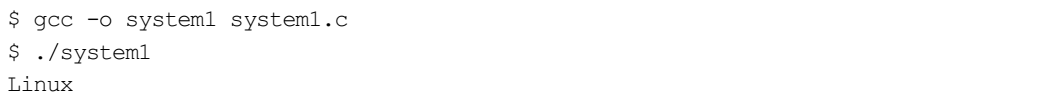
\includegraphics[scale=0.5]{images/lec07-pic19.png}
	\end{figure}
\end{frame}

\begin{frame}[fragile]
	\begin{minted}{c}
	#include <stdlib.h>
	#include <stdio.h>	
	int main(void)
	{
		system("sleep 5");
		fprintf(stderr, "end-of-program\n");
		return 0;
	}
	\end{minted}
	Работа функции system:
	\begin{figure}[h]
		\centering
		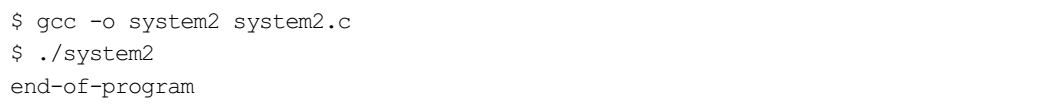
\includegraphics[scale=0.4]{images/lec07-pic21.png}
	\end{figure}
	\begin{itemize}
		\item system() ожидает завершения переданной ей команды. Поэтому сообщение "endof-program" выводится на экран примерно через 5 с;
		\item в system() можно передавать не только имя программы, но и аргументы.
	\end{itemize}
\end{frame}

\begin{frame}{Запуск нового процесса}
	В UNIX действие загрузки в память и запуска образа программы выполняется отдельно от операции по созданию нового процесса:
	\begin{itemize}
		\item один системный вызов (\textbf{exec}) загружает бинарную программу в память, замещая текущее содержание адресного пространства, и начинает выполнение новой программы. 
		\item другой системный вызов (\textbf{fork}) используется для создания нового процесса, который изначально является практически копией своего 	родительского.
	\end{itemize}
\end{frame}

\begin{frame}[fragile]{Системный вызов fork()}
	Новый процесс, запускающий тот же системный образ, что и текущий, может быть создан с помощью системного вызова \textbf{fork}():
	\begin{minted}{c}
	#include <sys/types.h>
	#include <unistd.h>	
	
	pid_t fork(void);
	\end{minted}
	\begin{itemize}
		\item В случае успешного обращения к \textit{fork}() создается новый процесс, во всех отношениях идентичный вызывающему. 
		\item Оба процесса выполняются от точки обращения к \textit{fork}(), как будто ничего не происходило.
	\end{itemize}
\end{frame}

\begin{frame}[fragile]{Пример fork()}
Программа:
	\begin{minted}{c}
#include <unistd.h>
#include <stdio.h>

int main (void)
{
    fork ();

    printf ("Hello World\n");

    sleep (15);
    
    return 0;
}
	\end{minted}
\end{frame}

\begin{frame}{Пример fork()}
	Результат:
	\begin{figure}[h]
		\centering
		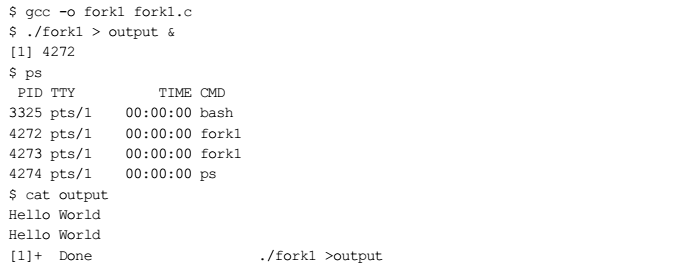
\includegraphics[scale=0.75]{images/lec07-pic32.png}
	\end{figure}
\end{frame}

\begin{frame}{Системный вызов fork()}
	В дочернем процессе успешный запуск \textbf{fork()} возвращает \textbf{0}. В родительском \textbf{fork()} возвращает \textbf{pid} дочернего. 
	~
	Родительский и дочерний процессы практически идентичны, за исключением некоторых особенностей:
	\begin{itemize}
		\item pid дочернего процесса назначается заново и отличается от родительского;
		\item родительский pid дочернего процесса установлен равным pid родительского процесса;
		\item ресурсная статистика дочернего процесса обнуляется;
		\item любые ожидающие сигналы прерываются и не наследуются дочерним процессом;
		\item никакие вовлеченные блокировки файлов не наследуются дочерним процессом.
	\end{itemize}
\end{frame}

\begin{frame}[fragile, shrink]{Пример fork()}
	Программа:
	\begin{minted}{c}
#include <sys/types.h>
#include <unistd.h>
#include <stdio.h>

int main (void)
{
    pid_t result = fork();
    if (result == -1) {
        fprintf (stderr, "Error\n");
        return 1;
    }
    if (result == 0)
        printf ("I'm child with PID=%d\n", getpid ());
    else
        printf ("I'm parent with PID=%d\n", getpid ());    
    return 0;
}
	\end{minted}
\end{frame}

\begin{frame}[fragile, shrink]{Переключения процессов}
	\begin{minted}{c}
#include <stdio.h>
#include <sys/types.h>
#include <unistd.h>
#include <time.h>

#define WORKTIME 3

int main (void)
{
    unsigned long parents = 0;
    unsigned long children = 0;

    pid_t result;    
    time_t nowtime = time (NULL);    
    result = fork ();    
    if (!result) 
    {
        while (time (NULL) < nowtime + WORKTIME) 
            children++;
        printf ("children: %ld\n", children);
    } 
    else 
    {
        while (time (NULL) < nowtime + WORKTIME) 
            parents++;
        printf ("parents: %ld\n", parents);
    }    
    return 0;
}
	\end{minted}
\end{frame}

\begin{frame}[fragile]
	В случае ошибки дочерний процесс не создается, fork() возвращает –1, устанавливая соответствующее значение errno. 
	~
	Вот два возможных значения errno и их смысл:
	\begin{itemize}
		\item EAGAIN — ядро не способно выделить определенные ресурсы, например новый pid, или достигнуто ограничение по ресурсам RLIMIT\_NPROC;
		\item ENOMEM — недостаточно ресурсов памяти ядра, чтобы завершить запрос.
	\end{itemize}
	\begin{minted}{c}
	pid_t pid;        
	pid = fork ();    
	if (pid > 0)        
		printf ("A parent process with cpid = %ld\n", pid);
	else if (pid == 0)
		printf ("A child process\n");
	else /*pid < 0*/
		perror("fork");	
	\end{minted}
\end{frame}

\begin{frame}[fragile]
	Чаще всего системный вызов fork() используется для создания нового процесса и последующей загрузки в него нового двоичного образа.  Сначала процесс ответвляет новый процесс, а потом дочерний процесс создает новый двоичный образ.
	\begin{minted}{c}
	pid_t pid;
    
	pid = fork ();
    
	if (pid == -1)
		perror("fork");
	if (pid == 0) {
		const char *args[] = {"ls", "/", NULL};
		execv("ls", args);
		perror("execv");
		exit(EXIT_FAILURE);
	}
	\end{minted}
\end{frame}

\begin{frame}{Семейство вызовов exec}
Единой функции exec не существует; на одном системном вызове построено целое
семейство таких функций. Рассмотрим execl:
\begin{figure}[h]
\centering
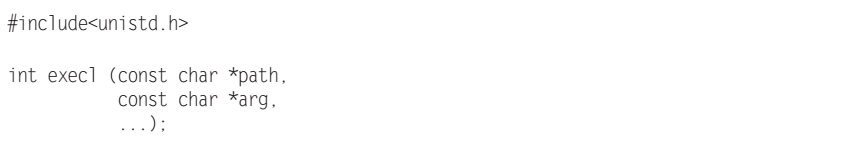
\includegraphics[scale=0.5]{images/lec07-pic04.png}
\end{figure}
\begin{itemize}
\item вызов execl() замещает текущий образ процесса новым, загружая в память
программу, определенную path. 
\item параметр arg — первый аргумент этой программы. 
\item Многоточие означает переменное количество аргументов — у функции
execl() их количество может быть любым
\item дополнительные аргументы можно указывать в скобках один за другим
\item список аргументов всегда завершается значением NULL.
\end{itemize}
\end{frame}

\begin{frame}{Семейство вызовов exec}
Следующий программный код замещает выполняющуюся в настоящий момент программу с /bin/vi:
\begin{figure}[h]
\centering
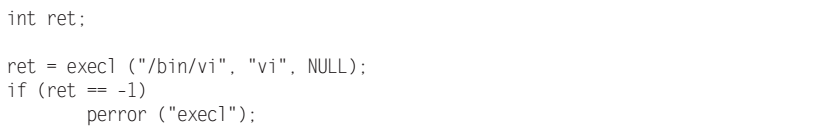
\includegraphics[scale=0.5]{images/lec07-pic05.png}
\end{figure}
Если вы хотите редактировать файл /home/kidd/hooks.txt, то должны запустить следующий код:
\begin{figure}[h]
\centering
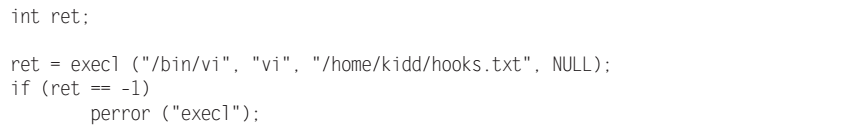
\includegraphics[scale=0.5]{images/lec07-pic06.png}
\end{figure}
\end{frame}

\begin{frame}{Семейство вызовов exec}
\begin{itemize}
\item при успешном вызове execl() не возвращает никаких значений 
\item если произошла ошибка, execl() возвращает –1 и устанавливает errno.
\end{itemize}
В случае успешного выполнения вызов execl():
\begin{itemize}
\item изменяет адресное пространство и образ процесса;
\item любые ожидающие сигналы исчезают;
\item любые сигналы, отлавливаемые процессом, возвращаются к своему
поведению по умолчанию;
\item все блокировки памяти удаляются;
\item большинство атрибутов потока возвращается к значениям по умолчанию;
\item большая часть статистических данных процесса сбрасывается;
\item все адресное пространство памяти, относящееся к данному процессу, включая
загруженные файлы, очищается.
\end{itemize}
\end{frame}

\begin{frame}{Семейство вызовов exec}
\begin{itemize}
\item execl, execlp, execle  
\item execv, execvp, execve
\end{itemize}
<<Расшифровка>> названий функций:
\begin{itemize}
\item \textbf{l} и \textbf{v} указывают, передаются ли аргументы списком или массивом. 
\item \textbf{p} указывает, что система будет искать указанный файл по
полному пользовательскому пути. 
\item \textbf{е} обозначает, что для нового процесса создается новое окружение.
\end{itemize}
\end{frame}

\begin{frame}{Семейство вызовов exec}
В прогремме образ текущего процесса заменяется программой
/bin/uname с опцией -a. Если программа была успешно вызвана (независимо от того,
как она завершилась), то сообщение "Error" не выводится. 
\begin{figure}[h]
\centering
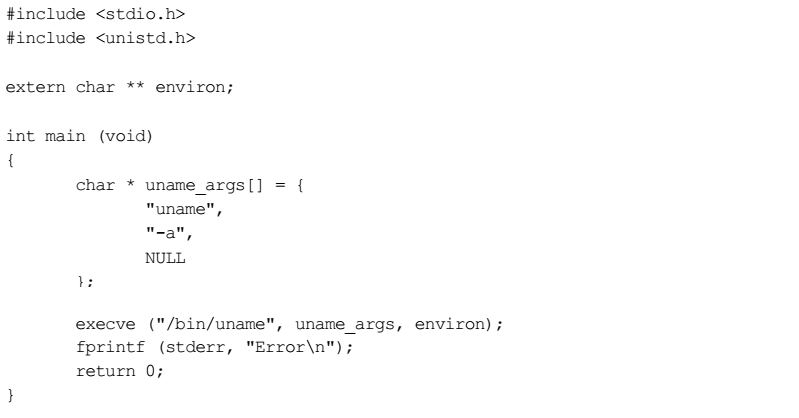
\includegraphics[scale=0.5]{images/lec07-pic36.png}
\end{figure}
\end{frame}

\begin{frame}{Пример: окружение, аргументы}
\begin{figure}[h]
\centering
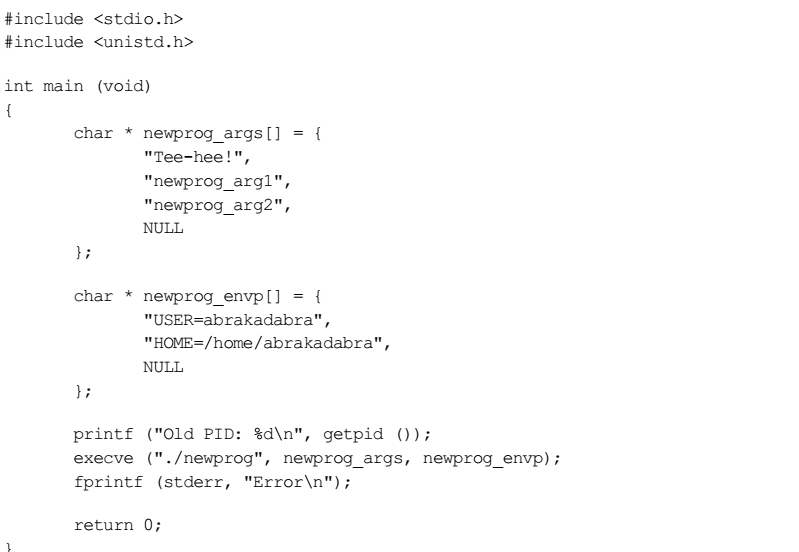
\includegraphics[scale=0.5]{images/lec07-pic37.png}
\end{figure}
\end{frame}

\begin{frame}{Пример: окружение, аргументы}
\begin{figure}[h]
\centering
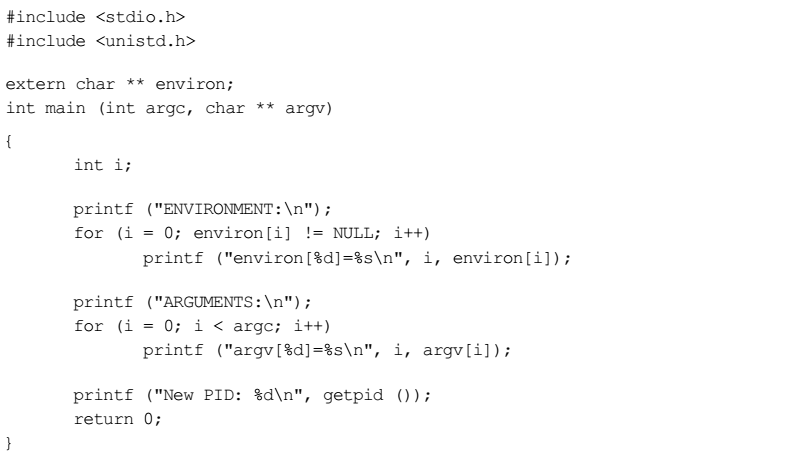
\includegraphics[scale=0.5]{images/lec07-pic38.png}
\end{figure}
\end{frame}

\begin{frame}{Пример: окружение, аргументы}
Результат:
\begin{figure}[h]
\centering
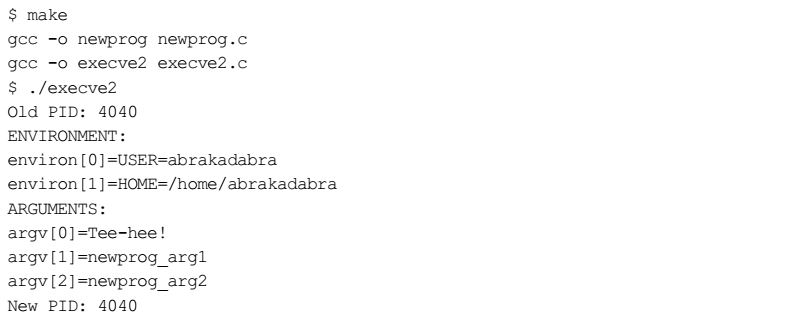
\includegraphics[scale=0.5]{images/lec07-pic39.png}
\end{figure}
Данный пример демонстрирует сразу три аспекта работы системного вызова
execve():
\begin{itemize}
\item обе программы выполнялись в одном и том же процессе;
\item при помощи системного вызова execve() программе можно "подсунуть" любое окружение;
\item в элементе argv[0] действительно может быть все, что угодно.
\end{itemize}
\end{frame}

\begin{frame}[fragile, shrink]
	\begin{minted}{c}
#include <stdio.h>
#include <unistd.h>
#include <sys/types.h>

extern char ** environ;

int main (void)
{
    pid_t result;
    char * sleep_args[] = {
        "sleep",
        "5",
        NULL
    };
    result = fork ();
    if (result == -1) {
        fprintf (stderr, "fork error\n");
        return 1;
    }
    if (result == 0) {
        execve ("/bin/sleep", sleep_args, environ);
        fprintf (stderr, "execve error\n");
        return 1;
    } 
    else 
        fprintf (stderr, "I'm parent with PID=%d\n", getpid());
    return 0;
}
	\end{minted}
\end{frame}

\begin{frame}{Пример: совместный вызов fork и exec}
Результат
\begin{figure}[h]
\centering
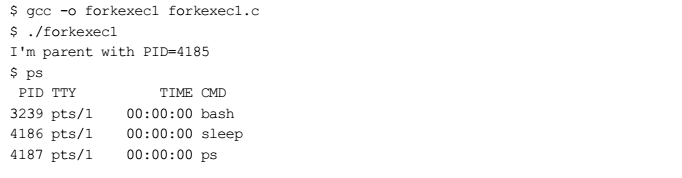
\includegraphics[scale=0.5]{images/lec07-pic41.png}
\end{figure}
\begin{itemize}
\item Программа породила новый процесс и запустила в нем программу
/bin/sleep, которая дает нам возможность в течение 15 с набрать команду ps и насладиться наличием в системе отдельного процесса.
\item Сообщение <<I'm parent with PID=...>> выводится в стандартный поток ошибок
(stderr), хотя фактически не является ошибкой. Это искусственный прием, позволяющий выводить сообщение на экран немедленно, не задумываясь о возможных
последствиях буферизации стандартного вывода.
\end{itemize}
\end{frame}

\section{Завершение процесса}

\begin{frame}{Завершение процесса}
	POSIX и C89 определяют следующую стандартную функцию для завершения текущего процесса:
	\begin{itemize}
		\item вызов exit() выполняет некоторые основные шаги перед завершением, а затем отправляет ядру команду прекратить процесс.
		\item параметр status используется для обозначения статуса процесса завершения.
		\item значения EXIT\_SUCCESS и EXIT\_FAILURE определяются в качестве способов представления успеха и неудачи. 
	\end{itemize}
	Перед тем как прервать процесс, библиотека C выполняет подготовительные шаги в следующем порядке.
	\begin{enumerate}
		\item Вызов всех функций, зарегистрированных с atexit() или on\_exit(), в порядке, обратном порядку регистрации.
		\item Сброс всех стандартных потоков ввода­вывода.
		\item Удаление всех временных файлов, созданных функцией tmpfile(). 
	\end{enumerate}
\end{frame}

\begin{frame}{Завершение процесса}
	Другие способы завершения:
	\begin{itemize}
		\item достижение конечной точки программы (системный выхов exit - неявный);
		\item полезно возвращать статус выхода явно;
		\item процесс также может завершиться, если ему отправлен сигнал, действие которого по умолчанию - окончание процесса (SIGTERM и 		SIGKILL);
		\item ядро может прервать процесс, выполняющий недопустимые инструкции, нарушающий сегментацию, исчерпавший ресурсы памяти и т. д.
\end{itemize}
\end{frame}

\begin{frame}[fragile]{atexit()}
	POSIX 1003.1­2001 определяет, а \textit{Linux} поддерживает библиотечный вызов \textbf{atexit}(), используемый для регистрации функций, вызываемых при завершении процесса:
	\begin{minted}{c}
	#include <stdlib.h>
	int atexit(void (*function)(void));
	\end{minted}
	\begin{itemize}
		\item При успешном срабатывании \textit{atexit}() регистрирует указанную функцию для запуска при нормальном завершении процесса, то есть с помощью системного вызова \textit{exit}() или возврата результатов функцией \textit{main}(). 
		\item Если процесс запускает функцию \textit{exec}, список зарегистрированных функций очищается (поскольку функции больше не существуют в новом адресном пространстве процесса). 
		\item Если процесс прерывается сигналом, зарегистрированные функции не вызываются.
	\end{itemize}
\end{frame}

\section{Ожидание завершения процесса}

\begin{frame}[fragile]{Ожилание завершения процесса}
	Процессы в \textit{Linux} работают независимо друг от друга, но иногда встает задача организации последовательного выполнения процессов.
	\begin{itemize}
		\item \textbf{Пример 1}: реализация последовательного выполнения процессов — ожидание родителем завершения своего потомка. Если мы запускаем программу не в фоновом режиме, то оболочка не выдаст приглашение командной строки до тех пор, пока данная программа не завершится.
		\item \textbf{Пример 2}: последовательный запуск родительским процессом двух и более потомков. Например, многие командные оболочки позволяют разделять несколько команд точкой с запятой, организовывая тем самым их последовательное выполнение: 
		\begin{alltt}
			> sleep 5 ; ls /
		\end{alltt}
\end{itemize}
\end{frame}

\begin{frame}[fragile, shrink]
	\begin{minted}{c}
#include <stdio.h>
#include <unistd.h>
#include <sys/types.h>

int main (void)
{
    pid_t result = fork ();
    if (result == -1) {
        fprintf (stderr, "Fork error\n");
        return 1;
    }
    /* Child */
    if (result == 0) {
        execlp ("ls", "ls", "/", NULL);
        fprintf (stderr, "Exec error\n");
        return 1;
    }    
    /* Parent */
    sleep (3);    
    fprintf (stderr, "I'm parent\n");    
    return 0;
}
	\end{minted}
\end{frame}

\begin{frame}
	Когда дочерний процесс завершается прежде родительского, ядро должно поместить потомка в особый процессный статус. 
	\begin{itemize}
		\item Процесс в этом состоянии известен как \textbf{зомби}. 
		\item В данном состоянии существует лишь «скелет» процесса — некоторые основные структуры данных, содержащие потенциально нужные 	сведения. 
		\item Процесс в таком состоянии ожидает запроса о своем статусе от предка (процедура, известная как ожидание процесса­зомби). 
		\item Только после того как предок получит всю необходимую информацию о завершенном дочернем процессе, последний формально удаляется и перестает существовать даже в статусе зомби.
	\end{itemize}
\end{frame}

\begin{frame}[fragile]
Ядро Linux предоставляет несколько интерфейсов для получения информации о завершенном дочернем процессе. Самый простой из них, определенный POSIX, называется wait(): 
	\begin{minted}{c}
	#include <sys/types.h>
	#include <sys/wait.h>	
	pid_t wait(int *status);
	\end{minted}
	\begin{itemize}
		\item Вызов wait() возвращает pid завершенного дочернего процесса или –1 в случае ошибки. 
		\item Если никакого дочернего процесса не было прервано, вызов блокируется, пока потомок не завершится. 
		\item Если дочерний процесс уже был завершен, вызов возвращает результаты немедленно. 
	\end{itemize}
	В случае ошибки возможно присвоение переменной errno одного из двух значений:
	\begin{itemize}
		\item ECHILD - вызывающий процесс не имеет дочерних;
		\item EINTR - сигнал был получен во время ожидания, в результате чего вызов вернул результат слишком рано.
	\end{itemize}
\end{frame}

\begin{frame}[fragile, shrink]
	\begin{minted}{c}
#include <stdio.h>
#include <wait.h>
#include <unistd.h>
#include <sys/types.h>

int main (int argc, char ** argv)
{
    pid_t status, childpid;   
    int exit_status;    
    if (argc < 2) {
        fprintf (stderr, "Too few arguments\n");
        return 1;
    }
    status = fork ();
    if (status == -1) {
        fprintf (stderr, "Fork error\n");
        return 1;
    }    
    if (status == 0) { /* Child */
        execlp ("ls", "ls", argv[1], NULL);
        fprintf (stderr, "Exec error\n");
        return 1;
    }    
    childpid = wait (&exit_status); /* Parent */
    if (WIFEXITED (exit_status)) {
        printf ("Process with PID=%d "
            "has exited with code=%d\n", childpid,
            WEXITSTATUS (exit_status));
    } 
    return 0;
}
	\end{minted}
\end{frame}

\begin{frame}[fragile, shrink]
	В случае ошибки возможно присвоение переменной errno одного из двух значений:
	\begin{itemize}
		\item ECHILD - вызывающий процесс не имеет дочерних;
		\item EINTR - сигнал был получен во время ожидания, в результате чего вызов вернул результат слишком рано.
	\end{itemize}
	Если указатель status не содержит значения NULL, там находится дополнительная информация о дочернем процессе. 
	\begin{minted}{c}
	#include <sys/wait.h>	
	WIFEXITED(status);
	WIFSIGNALED(status);
	WIFSTOPPED(status);
	WIFCONTINUED(status);
	WIFCONTINUED(status);	
	WIFCONTINUED(status);
	WEXITSTATUS(status);	
	WTERMSIG(status);		
	WSTOPSIG(status);			
	WCOREDUMP(status);
	\end{minted}
\end{frame}

\begin{frame}
	Статус завершившегося потомка — это целое число, содержащее код возврата и некоторую другую информацию о том, как завершился процесс.
	\begin{itemize}
		\item WIFEXITED() - возвращает ненулевое значение, если потомок завершится посредством возврата из функции main() или через вызов exit().
		\item WEXITSTATUS() - возвращает код возврата завершившегося процесса. Этот макрос вызывается в том случае, если WIFEXITED() вернул ненулевое значение.
		\item WIFSIGNALED() - возвращает ненулевое значение, если процесс был завершен посредством получения сигнала. 
		\item WTERMSIG(), WCOREDUMP(), WIFSTOPPED(), WSTOPSIG() и WCONTINUED() - относятся к сигналам (будут рассмотрены в следующей лекции).
	\end{itemize}	
\end{frame}

\begin{frame}
	\begin{figure}[h]
		\centering
		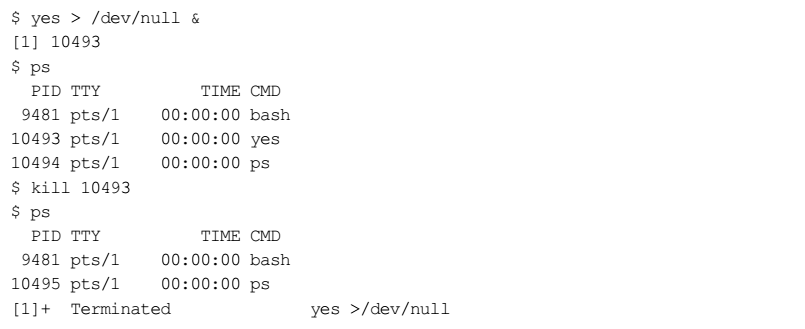
\includegraphics[scale=0.6]{images/lec07-pic42.png}
	\end{figure}
\end{frame}

\begin{frame}[fragile, shrink]
	\begin{minted}{c}
#include <stdio.h>
#include <wait.h>
#include <unistd.h>
#include <sys/types.h>

int main (void)
{
    pid_t status, childpid;    
    int exit_status;    
    status = fork ();    
    if (status == -1) {
        fprintf (stderr, "Fork error\n");
        return 1;
    }
	/* Child */
    if (status == 0) {
        execlp ("sleep", "sleep", "30", NULL);
        fprintf (stderr, "Exec error\n");
        return 1;
    }
    /* Parent */
    childpid = wait (&exit_status);    
    if (WIFEXITED (exit_status)) {
        printf ("Process with PID=%d "
            "has exited with code=%d\n", childpid,
            WEXITSTATUS (exit_status));
    }
    if (WIFSIGNALED (exit_status)) {
        printf ("Process with PID=%d "
        "has exited with signal.\n", childpid);
    }    
    return 0;
}
	\end{minted}
\end{frame}

\begin{frame}[fragile]{Ожидание определенного процесса}
	Если необходимо ожидать завершения дочернего процесса, можно использовать системный вызов \textbf{waitpid()}:
	\begin{minted}{c}
	#include <sys/types.h>
	#include <sys/wait.h>
	
	pid_t waitpid(pid_t pid, int *status, int options);
	\end{minted}
	Параметр pid точно определяет:
	\begin{itemize}
		\item $< -1$ -- ожидание любого дочернего процесса, чей ID группы процессов равен абсолютному значению этой величины;
		\item $-1$ -- ожидание любого дочернего процесса; поведение аналогично \textit{wait}();
		\item $0$ -- ожидание любого дочернего процесса, принадлежащего той же группе процессов, что и вызывающий;
		\item $>0$ -- ожидание любого дочернего процесса, чей \textit{pid} в точности равен указанной величине.
	\end{itemize}
\end{frame}

\section{Демоны}

\begin{frame}{Демон}
	\begin{block}{Демон}
		процесс, который запущен в фоновом режиме и не привязан ни к какому управляющему терминалу.
	\end{block}
	Демоны обычно запускаются во время загрузки с правами \textit{root} или другими специфическими пользовательскими правами (например, \textit{apache} или \textit{postfix}) и выполняют задачи системного уровня. 
	\begin{itemize}
		\item демон должен запускаться как потомок процесса \textit{init};
		\item демон не должен быть связан с терминалом.
	\end{itemize}
\end{frame}

\begin{frame}
	\begin{figure}[h]
		\centering
		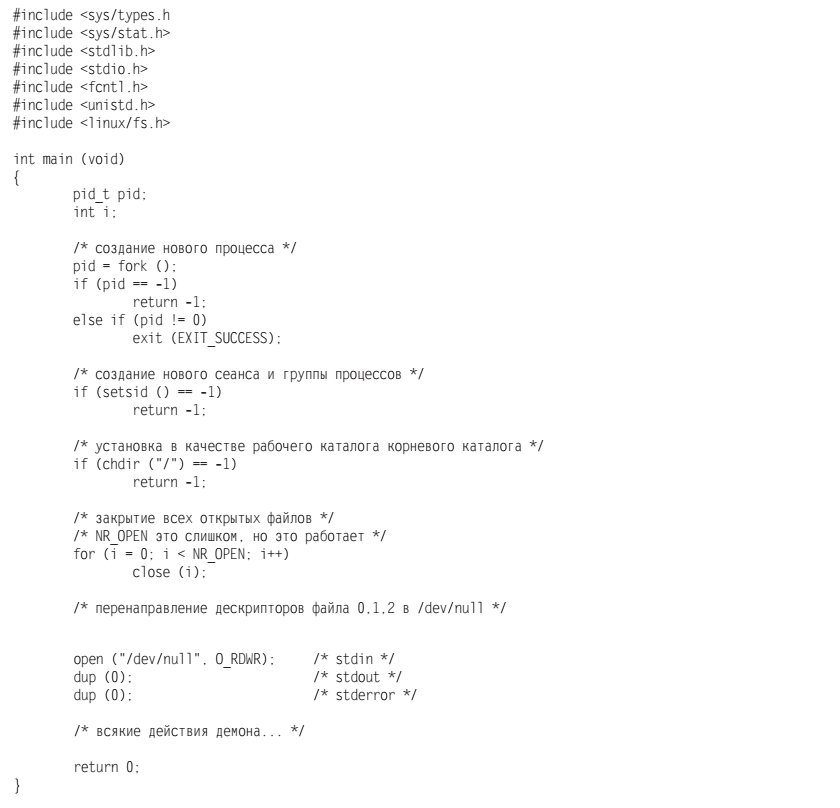
\includegraphics[scale=0.4]{images/lec07-pic16.png}
	\end{figure}
\end{frame}

\end{document}